\documentclass{scrartcl}
\usepackage[latin1]{inputenc}
\usepackage[T1]{fontenc}
\usepackage[ngerman]{babel}
\usepackage{amsmath}
\usepackage{amssymb}
\usepackage{icomma}
\usepackage{nicefrac}
%\usepackage[dvips]{graphicx}
%\usepackage{floatflt}
%\usepackage{enumitem}
%\usepackage{babel}
\usepackage{blindtext}
%\usepackage{showframe}
\usepackage{calc}
\usepackage{wrapfig}
\def\BILD{\rule{0.4\textwidth}{4cm}}

\usepackage{graphicx}
\usepackage{placeins}
\usepackage{multirow}
\usepackage{subfig}
\usepackage{url}

\renewcommand{\topfraction}{.85}
\renewcommand{\bottomfraction}{.7}
\renewcommand{\textfraction}{.15}
\renewcommand{\floatpagefraction}{.66}
\renewcommand{\dbltopfraction}{.66}
\renewcommand{\dblfloatpagefraction}{.66}
\setcounter{topnumber}{9}
\setcounter{bottomnumber}{9}
\setcounter{totalnumber}{20}
\setcounter{dbltopnumber}{9}
\setlength{\intextsep}{0cm plus1cm minus1cm}
\setlength{\parindent}{0cm}
\pdfminorversion = 5
\usepackage{setspace}
\onehalfspacing

\begin{document}
\title{Versuch 11: Atomspektren}

\date{\today}

\author{Gruppe 5a: Gia-Danh Lam, Nils Haldenwang}

\maketitle
\tableofcontents

\newpage
\section{Einleitung und theoretischer Hintergrund}
\label{sec:einleitung}

\section{Aufgaben}
\subsection{Bestimmung des Planck'schen Wirkungquantums}
\begin{figure}%

\includegraphics[width=14cm]{pics/dummypic}%
\caption{Versuchsaufbau}%
\label{pic:2}%
\end{figure}
Dieser Versuch befasst sich mit dem photoelektrischem Effekt. Dazu wird eine Photozelle mit verschiedenem Licht beleuchtet und jeweils die Grenzspannung $U_0$ bestimmt. Der Aufbau ist in Abbildung 1 dargestellt. Es wird eine Quecksilberlampe als Lichtquelle verwendet. In einem V-f�rmigen Kasten wird der Lichtstrahl gebrochen und dadurch entsteht das charakteristische Linienspektrum von Quecksilber, das am anderen Ende des Kastens durch einen Spiegel in die andere Richtung umgelenkt wird. In der Tabelle \ref{tab:1} sind diese aufgelistet.
\begin{table}%[htb!]
	\begin{tabular}{|l|lllll|}
	\hline
	Farbe& gelb& gr�n& gr�nblau&blau-violett&tief violett\\
	\hline
	Frequenz (THz)&518,7&549,1&609,3&689,2&740,2\\
	\hline
	\end{tabular}
\caption{im Versuch beobachtbares Linienspektrum von Quecksilber}
\label{tab:1}
\end{table}
Der andere Teil des Kastens ist drehbar, sodass die Photozelle, die in diesem Kasten fixiert ist, auf einen der Lichtstrahlen gerichtet werden kann. Um die Grenzspannung zu bestimmen, werden zwei Methoden verwendet, wobei bei der zweiten Methode die Einstellung der Photozelle nach Augenma� vorgenommen wurde. Bei der ersten Methode haben wir mithilfe des Strommessers die Stelle bestimmt, bei der der Photostrom ihr Maximum annahm.
\subsection{Messmethode mit Anlegen einer Gegenspannung}

\label{sec:gegenspannung}
\begin{figure}%
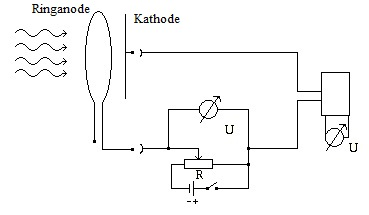
\includegraphics[width=10cm]{pics/photozelle}%
\caption{Schaltung zur Photozelle}%
\label{pic:3}%
\end{figure}
In diesem Teil des Versuches wird eine Gegenspannung angelegt, die mithilfe eines Drehpotentiometers langsam und stetig erh�ht wird. Der Verlauf des Photostromes $I_{Ph}$ wird von einem Programm aufgezeichnet. Wenn die Gegenspannung gro� genug ist, treffen keine Elektronen mehr auf die Anode, sodass der Photostrom null wird. In den Aufzeichnung wird der Photostrom �ber die Gegenspannung aufgetragen, sodass das Ablesen der Grenzspannung m�glich ist (s. Anhang). Da die Erh�hung der Gegenspannung manuell geschehen ist, ist die Auftragung der Gegenspannung nicht linear, sodass das Ablesen der Gegenspannung nicht genau ist. Zu den in der Tabelle \ref{tab:1} genannten Lichtern werden die Grenzspannungen bestimmt (s.Tabelle \ref{tab:2}).
\begin{table}%[htb!]
	\begin{tabular}{|l|l|l|l|l|l|}
	\hline
	Grenzspannung in V&0,7 & 0,8 &1,0 &1,3 &1,5\\
	\hline
	 Frequenz (THz)&518,7 &549,1 &609,3 &689,2 & 740,2\\
	\hline
	\end{tabular}
\caption{Grenzspannung mit der jeweiligen Frequenz des Lichtes}
\label{tab:2}
\end{table}
Die Energien, die man durch Multiplikation von Grenzspannung und der Elementarladung $e$ erh�lt, sind �ber die Frequenz in Abbildung \ref{pic:4} dargestellt. F�r den Ablesefehler haben wir 0,05V angenommen, sodass die Werte in der Abbildung einen Fehler von $\Delta eU_0=0,05J\cdot1,6=0,08J$. Durch lineare Regression erhalten wir die Steigung $m_{f(x)}=(5,8\pm0,7)\cdot 10^{-34} Js$, wobei die Zehnerpotenzen der Elementarladung und der Frequenz mitber�cksichtigt worden sind. Der Fehler ist durch den maximal und minimal m�glichen Anstieg bestimmt worden. Nach der Gleichung \ref{eq:3} sollte die Steigung den Wert des Planck'schen Wirkungquantums annehmen, jedoch betr�gt der Literaturwert  $6,626 \cdot 10^{-34} Js$ und ist damit viel gr��er als der von uns ermittelte Wert. Bei der zweiten Messmethode erhielten wir �hnliche bzw. identische Ergebnisse f�r die Grenzspannung. Daher vermuten wir, dass ein systematischer Fehler zu diesem Ergebnis gef�hrt hat. Wo genau der statistische Fehler zu finden ist, k�nnen wir nicht sagen. Da aber bei beiden Messmethoden verschiedene Ger�te benutzt wurden, denken wir, dass das Problem wahrscheinlich durch die Photozelle entstanden ist. 
\begin{figure}%
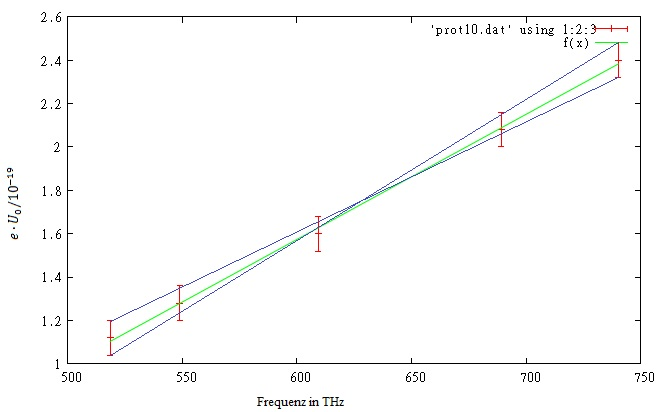
\includegraphics[width=15cm]{pics/gegen}%
\caption{grafische Auswertung der Messwerte zur ersten Messmethode mit der Gegenspannung}%
\label{pic:4}%
\end{figure}

\subsection{Messmethode mithilfe eines Elektrometers}

\begin{figure}%
	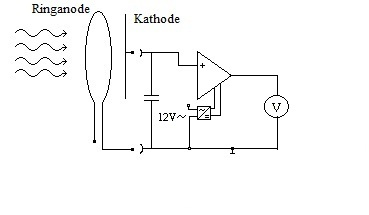
\includegraphics[width=10cm]{pics/photozelle2}%
	\caption{Schaltung zur Photozelle}%
	\label{pic:5}%
\end{figure}
Bei der zweiten Messmethode wird ausgenutzt, dass ohne Anlegen einer Gegenspannung eine Spannung zwischen der Anode und der Kathode aufgebaut wird, die der Grenzspannung entspricht. Dadurch wird ein Kondensator geladen (s. Abbildung \ref{pic:4}). Die Spannung wird mit einem Multimeter gemessen. Die gemessenen Werte f�r die Grenzspannungen sind in der Tabelle \ref{tab:3} dargestellt. 
\begin{table}[htb!]%
	\begin{tabular}{|l|l|l|l|l|l|}
	\hline
	Grenzspannung in V&0,7 & 0,8 &0,95 &1,35 &1,45\\
	\hline
	 Frequenz (THz)&518,7 &549,1 &609,3 &689,2 & 740,2\\
	\hline
	\end{tabular}
\caption{Grenzspannung mit der jeweiligen Frequenz des Lichtes}
\label{tab:3}
\end{table}
Auch hier wird durch lineare Regression die Steigung bestimmt, die hier $m_{h(x)}=(5,7\pm1,1)\cdot 10^{-34} Js$ betr�gt (s.Abbildung \ref{pic:6}). Da bei dieser Methode das Richten der Photozelle auf eine der Lichter relativ ungenau geschehen ist, nehmen wir einen Fehler von 0,1V an, sodass $\Delta eU_0=0,1J\cdot1,6=0,16J$ gro� ist. Der Fehler f�r die Steigung wurde nach der gleichen Methode wie in \ref{sec:gegenspannung} bestimmt. Auch hier ist die Steigung viel kleiner als der Literaturwert $6,626 \cdot 10^{-34} Js$ und wie schon oben genannt, ist der systematische Fehler wahrscheinlich mit der Photozelle verbunden.
\begin{figure}%
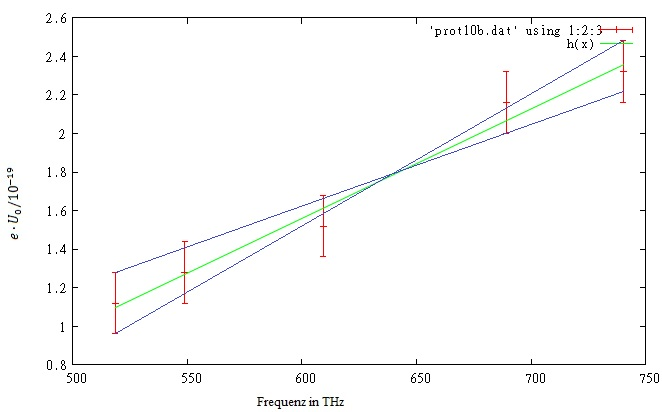
\includegraphics[width=15cm]{pics/feld}%
\caption{grafische Auswertung der Messwerte zur ersten Messmethode mit dem Elektrometer}%
\label{pic:6}%
\end{figure}

\section{Fazit}
\label{sec:fazit}



\end{document}



